\chapter{Background}
This chapter provides a brief technical overview of the models that we will frequently encounter in the rest of the thesis. A fundamental understanding of these systems is essential for appreciating the problems associated with them and the potential solution for overcoming those problems, which will be discussed in the subsequent chapters.

\section{RNN - A non linear dynamical system}
We frequently encounter data that is temporal in nature. A few obvious examples would  be, audio signals, videos signals, time series of a stock price and natural language (the holy grail of AI!). While traditional feed-forward neural networks are excellent at non linear curve fitting and classification tasks, it is unclear as to how they will approach the problem of predicting the value of a temporal signal $T$ at time $t$ given the states $T_{0}, T_{1}....T_{t-1}$ such that the states over time are not i.i.d. Human beings solve such problems by compressing and storing the previous states in memory and then using that information for predicting the state $T_t$. A conventional feed-forward network such as a MLP is inherently memoryless.

Recurrent neural networks overcome this restriction by having feedback loops which allow information to be carried from the current time step to the next. While the notion of implementing memory via feedback loops might seem daunting at first the architecture is refreshingly very simple. In a process known as unrolling a RNN can be seen as a sequence of MLPs (at different time steps) stacked together. More specifically, RNN maintains a memory across time-steps by projecting the information at any given time step $t$ onto a hidden(latent) state through parameters $\theta$ which are shared across different time-steps. Fig \ref{bck:rnn} shows a rolled and unrolled recurrent network.

\begin{figure}
	\begin{minipage}[t]{\textwidth}
		\ifpdf
		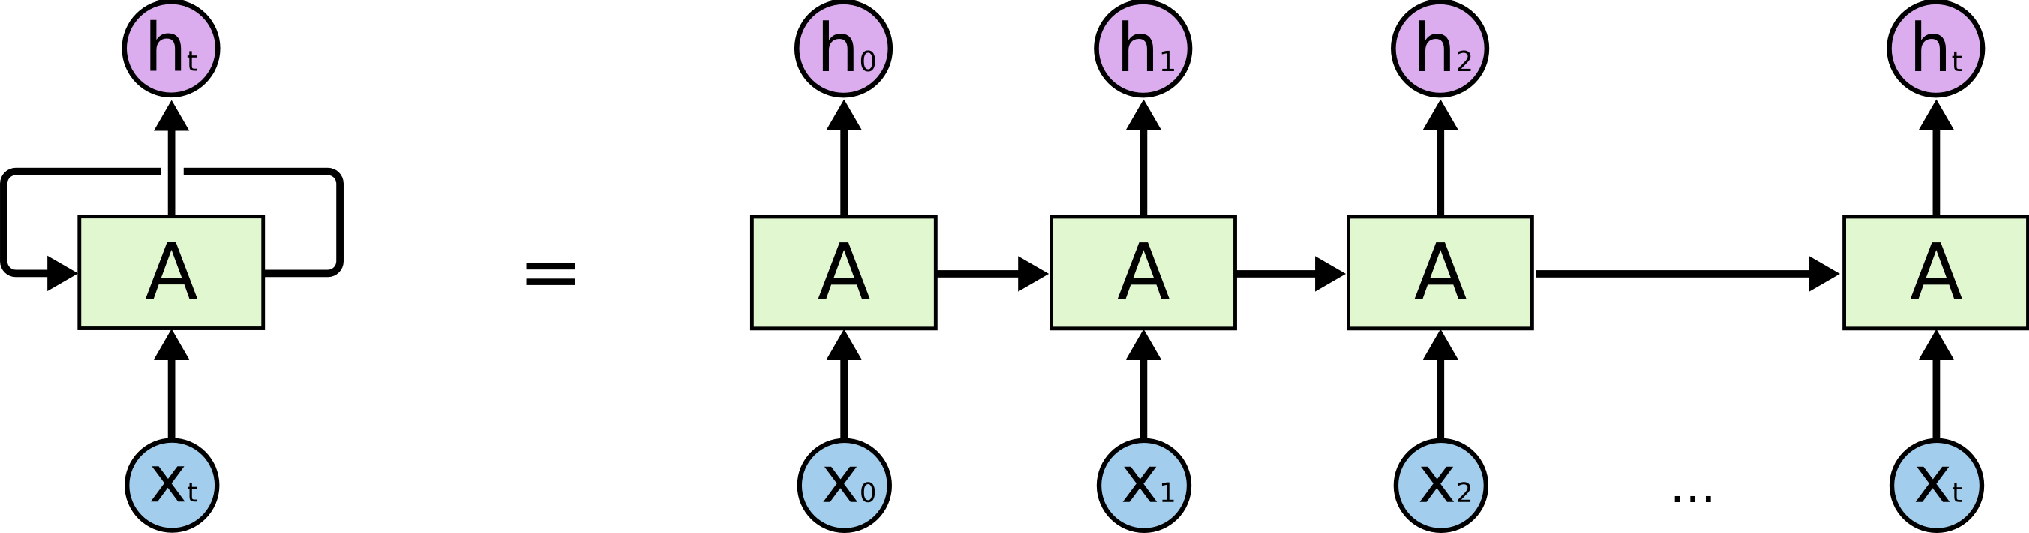
\includegraphics[width=\linewidth,keepaspectratio=true]{./figs/RNN-unrolled-pdf}
		\else
		\includegraphics[width=\linewidth,keepaspectratio=true]{./figs/RNN-unrolled-eps}
		\fi
		\caption{\small Schematic of a RNN \cite{olah}}
		\label{bck:rnn}
	\end{minipage}
\end{figure}

\subsection{Non linear dynamics inside a RNN cell}
equations\\
presence of strange attractors.

\begin{equation}\label{ndq}	
	h^{(t)} = f(x^{(t)}, h^{(t-1)})
\end{equation}

\begin{equation}
c_t = tanh(Ux_t + Wc_{t-1})
\end{equation}

\begin{equation}
y_t = sotmax(Vc_t)
\end{equation}


\section{BPTT and Vanishing Gradients}
The optimization step i.e. the backward pass over the network weights is not just with regards to the parameters at the final time step but over all the time steps across which the weights (parameters) are shared. This is known as Back Propagation Through Time (BPTT) and it gives rise to the problem of vanishing (or exploding) gradients in vanilla RNNs. This concept is better elaborated upon through equation in the following section.

\subsection{BPTT for Vanilla RNN}
\begin{equation}
\mathbf{\mathcal{L}\left(x,y\right)} = - \sum_{t}\left(y_t \log\hat{y_t}\right)
\end{equation}

%\begin{equation}
%\frac{\partial \mathbf{\mathcal{L}}}{\partial \alpha_t} = -\left(y_t-z_t\right)
%\end{equation}
Since the weight $W_{oh}$ is shared across all time steps, adding the derivatives across the sequence we get:

\begin{equation}
\frac{\partial \mathbf{\mathcal{L}}}{\partial W_{oh}} = \sum_{t}\frac{\partial \mathbf{\mathcal{L}}}{\partial \hat{y_t}} \frac{\partial  \hat{y_t}}{\partial W_{oh}}
\end{equation}

%\begin{equation}
%\frac{\partial \mathbf{\mathcal{L}}}{\partial b_z} = \sum_{t}\frac{\partial \mathbf{\mathcal{L}}}{\partial z_t} %\frac{\partial  z_t}{\partial b_z}
%\end{equation}
Now for time-step t $\rightarrow$ t+1:

\begin{equation}
\frac{\partial \mathbf{\mathcal{L}}\left(t+1\right)}{\partial W_{hh}} = \frac{\partial \mathbf{\mathcal{L}}\left(t+1\right)}{\partial \hat{y}_{t+1}} \frac{\partial  \hat{y}_{t+1}}{\partial \mathbf{h}_{t+1}} \frac{\partial \mathbf{h}_{t+1}}{\partial W_{hh}}
\end{equation}

Again since $W_{hh}$ is shared across time steps, the gradient at t+1 will have contribution from the previous time steps as well. Summing over all the time steps we get:

%\begin{equation}
%\frac{\partial \mathbf{\mathcal{L}}\left(t+1\right)}{\partial W_{hh}} = \frac{\partial %\mathbf{\mathcal{L}}\left(t+1\right)}{\partial \hat{y}_{t+1}} \frac{\partial  \hat{y}_{t+1}}{\partial \mathbf{h}_{t+1}} %\frac{\partial \mathbf{h}_{t+1}}{\partial \mathbf{h}_t} \frac{\partial \mathbf{h}_t}{\partial W_{hh}}
%\end{equation}

\begin{equation}
\frac{\partial \mathbf{\mathcal{L}}\left(t+1\right)}{\partial W_{hh}} = \sum_{\tau=1}^{t+1}\frac{\partial \mathbf{\mathcal{L}}\left(t+1\right)}{\partial \hat{y}_{t+1}} \frac{\partial  \hat{y}_{t+1}}{\partial \mathbf{h}_{t+1}} \frac{\partial \mathbf{h}_{t+1}}{\partial \mathbf{h}_{\tau}} \frac{\partial \mathbf{h}_{\tau}}{\partial W_{hh}}
\end{equation}

Aggregating over the whole sequence we get:

\begin{equation} \label{vanishing}
\frac{\partial \mathbf{\mathcal{L}}}{\partial W_{hh}} = \sum_{t}\sum_{\tau=1}^{t+1}\frac{\partial \mathbf{\mathcal{L}}\left(t+1\right)}{\partial \hat{y}_{t+1}} \frac{\partial  \hat{y}_{t+1}}{\partial \mathbf{h}_{t+1}} \frac{\partial \mathbf{h}_{t+1}}{\partial \mathbf{h}_{\tau}} \frac{\partial \mathbf{h}_{\tau}}{\partial W_{hh}}
\end{equation}

Looking at equation \ref{vanishing} we can see that the RNN gradient is a recursive product of $\frac{\partial h_t}{\partial h_{t-1}}$ and \textbf{in the event of this derivative being $\ll 1$ or $\gg 1$, the RNN gradient would vanish or explode respectively} when the network is trained over longer time-steps. In the former case the training would freeze while in the latter it would never converge. Therefore a vanilla RNN can't keep track of long term dependencies which is critical for tasks such as speech synthesis, music composition etc. The architectural modifications which solved the vanishing gradient problem and are the current de-facto RNN cell(s) are presented in the next section.

\iffalse
\begin{equation}
\frac{\partial \mathbf{\mathcal{L}}\left(t+1\right)}{\partial W_{hx}} = \frac{\partial \mathbf{\mathcal{L}}\left(t+1\right)}{\partial \mathbf{h}_{t+1}} \frac{\partial \mathbf{h}_{t+1}}{\partial W_{hx}}
\end{equation}

\begin{equation}
\begin{split}
\frac{\partial \mathbf{\mathcal{L}}\left(t+1\right)}{\partial W_{hx}} & = \frac{\partial \mathbf{\mathcal{L}}\left(t+1\right)}{\partial \mathbf{h}_{t+1}} \frac{\partial \mathbf{h}_{t+1}}{\partial W_{hx}} + \frac{\partial \mathbf{\mathcal{L}}\left(t+1\right)}{\partial \mathbf{h}_t} \frac{\partial \mathbf{h}_t}{\partial W_{hx}} \\
& = \frac{\partial \mathbf{\mathcal{L}}\left(t+1\right)}{\partial \mathbf{h}_{t+1}} \frac{\partial \mathbf{h}_{t+1}}{\partial W_{hx}} + \frac{\partial \mathbf{\mathcal{L}}\left(t+1\right)}{\partial \mathbf{h}_{t+1}} \frac{\partial \mathbf{h}_{t+1}}{\partial \mathbf{h}_t}\frac{\partial \mathbf{h}_t}{\partial W_{hx}}
\end{split}\end{equation}

\begin{equation}
\frac{\partial \mathbf{\mathcal{L}}\left(t+1\right)}{\partial W_{hx}} = \sum_{\tau=1}^{t+1} \frac{\partial \mathbf{\mathcal{L}}\left(t+1\right)}{\partial \mathbf{h}_{t+1}} \frac{\partial \mathbf{h}_{t+1}}{\partial \mathbf{h}_{\tau}} \frac{\partial \mathbf{h}_{\tau}}{\partial W_{hx}}
\end{equation}

\begin{equation}
\frac{\partial \mathbf{\mathcal{L}}}{\partial W_{hx}} = \sum_{t} \sum_{\tau=1}^{t+1} \frac{\partial \mathbf{\mathcal{L}}\left(t+1\right)}{\partial \hat{y}_{t+1}} \frac{\partial \hat{y}_{t+1}}{\partial \mathbf{h}_{t+1}} \frac{\partial \mathbf{h}_{t+1}}{\partial \mathbf{h}_{\tau}} \frac{\partial \mathbf{h}_{\tau}}{\partial W_{hx}}
\end{equation}
\fi

\section{Gated RNNs}
Looking at equation \ref{ndq} we can see that RNN is an example of an iterated function and can therefore exhibit complex and chaotic behavior(substantiate this in later sections). However if for instance the RNN was to compute an identity function then the gradient computation wouldn't vanish or explode since the Jacobian is simply an identity matrix (rephrase this and substantiate with equation/previous equations). Now while an identity initialization of recurrent weights by itself isn't very interesting it brings us to the underlying principle behind gated architectures i.e. the mapping from memory state at one time step to the next is close to identity function.

\begin{figure}[ht] 
	\begin{subfigure}[b]{0.5\linewidth}
		\centering
		\ifpdf
		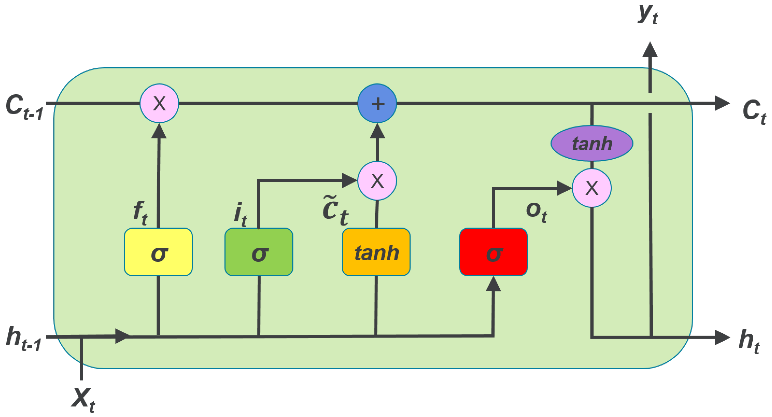
\includegraphics[width=0.95\linewidth]{./figs/Lstm-pdf}
		\else
		\includegraphics[width=0.95\linewidth]{./figs/Lstm-eps}
		\fi
		\caption{LSTM} 
		\label{lstm} 
		\vspace{4ex}
	\end{subfigure}%% 
	\begin{subfigure}[b]{0.5\linewidth}
		\centering
		\ifpdf
		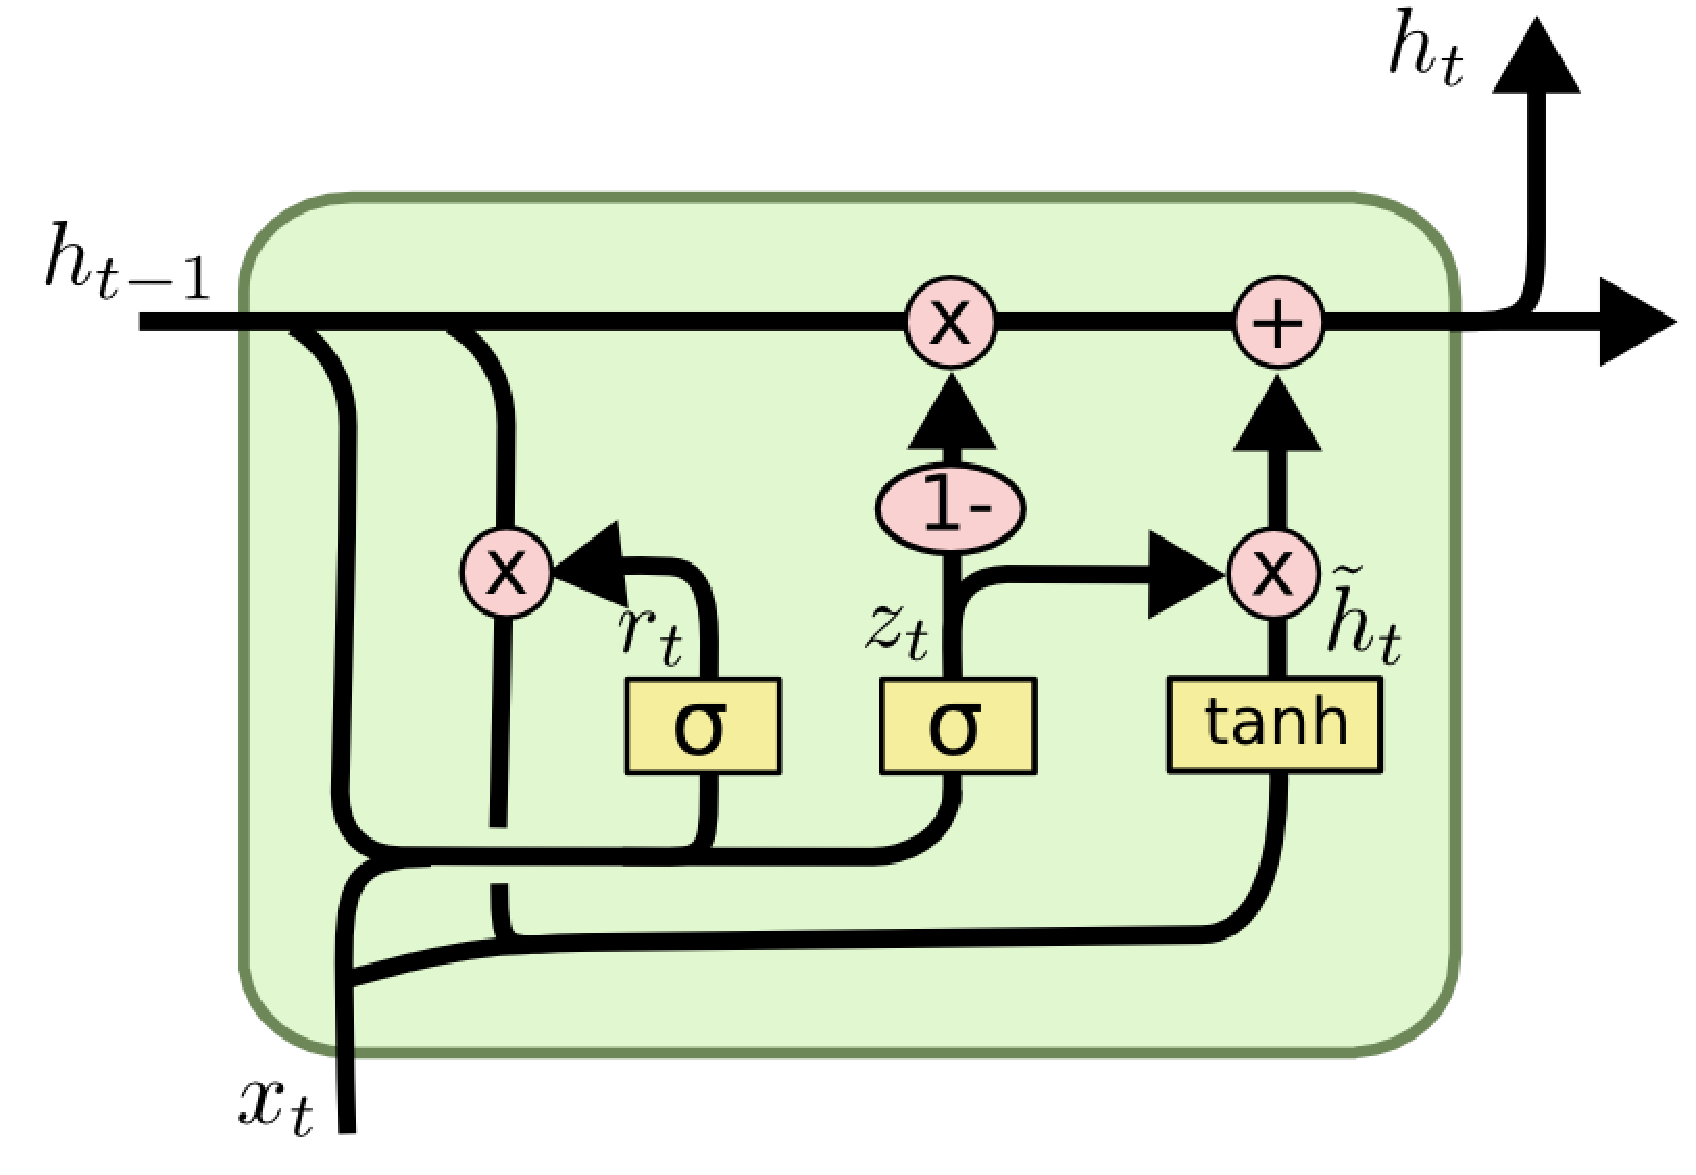
\includegraphics[width=0.95\linewidth]{./figs/Gru-pdf}
		\else
		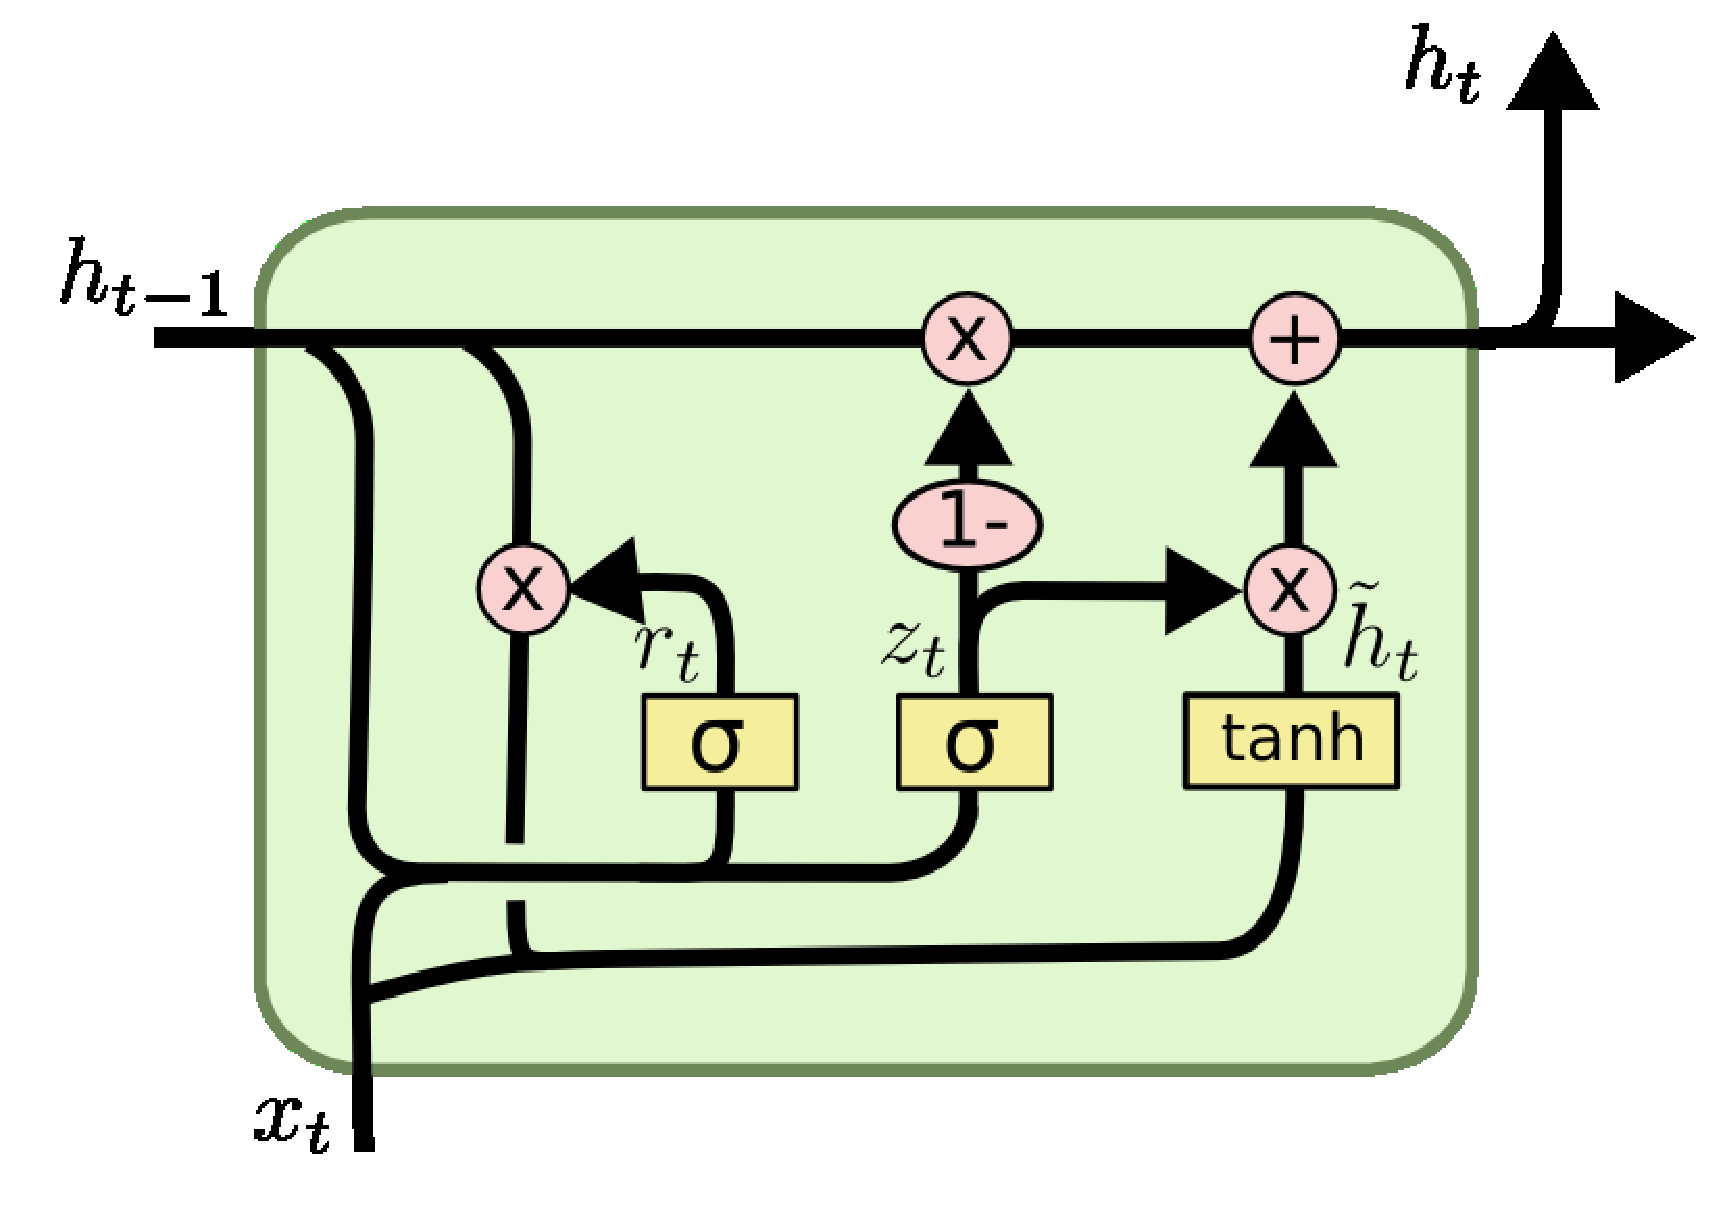
\includegraphics[width=0.95\linewidth]{./figs/Gru-eps}
		\fi 
		\caption{GRU} 
		\label{gru} 
		\vspace{4ex}
	\end{subfigure}
	\caption{Gated RNNs}
	\label{conf}
\end{figure}

\subsection{LSTM}
Long Short Term Memory (LSTM) introduced by \cite{LSTM} is one of the two most widely used gated RNN architectures in use today. The fact that it has survived all the path-breaking innovations in the field of deep learning for over twenty years to still be the state of the art in sequence modeling speaks volumes about the architecture's ingenuity and strong fundamentals. 

The fundamental principle behind the working of a LSTM is alter the memory vector only selectively between time steps such that the memory state is preserved over long distances (write this better). The architecture is explained as follows:


\begin{equation}
i= \sigma(x_t U^{(i)} m_{t-1}W^{(i)})
\end{equation}

\begin{equation}
f= \sigma(x_t U^{(f)} m_{t-1}W^{(f)})
\end{equation}

\begin{equation}
o= \sigma(x_t U^{(o)} m_{t-1}W^{(o)})
\end{equation}

\begin{equation}
\widetilde {c_t}= \tanh(x_t U^{(g)} m_{t-1}W^{(g)})
\end{equation}

\begin{equation}
c_t = c_{t-1} \odot f + \widetilde{c_t} \odot i
\end{equation}

\begin{equation}
m_t = tanh(c_t) \odot o
\end{equation}

The hidden state of a LSTM cell is the output which is then multiplied with the output weights followed by the softmax operation in order to yield the final output. The cell state is the memory of the LSTM unit. Furthermore the sigmoid activation for each one of the input, forget and output gates serves as a switch such that multiplying them element wise with other vector decides how much of the vector to filter out.
\begin{itemize}
	\item \textbf{input modulation gate $g^{(t)}$:} The input modulation gate is computed based on the present input and the previous hidden state (which is exposed to the output). It yields a candidate memory for the cell state. Since it doesn't determine how much of a particular information to retain, it doesn't have the sigmoid activation. The tanh layer serves the purpose of creating candidate memories for the new cell state.
	\item \textbf{input gate $i^{(t)}$:} The input first computes a new cell state based on the new input and the previous hidden state and then decides how much of this information to "let through". A sum of the hadamard products of the (input gate,modulation gate) and (forget gate, previous cell state) tuples respectively yields the new cell state.
	\item \textbf{forget gate $f^{(t)}$:} The forget gate decides what to remember and what to forget for the new memory based on the current input and the previous hidden state.The sigmoid activation acts like a switch where 1 implies remember everything while 0 implies forget everything.
	\item \textbf{output gate $o^{(t)}$:} A tanh on the new cell state yields the candidate hidden state. The output gate then determines determines how much of this internal memory to expose to the top layers (and subsequent timesteps) of the network.
\end{itemize}

\subsection{GRU}
The GRU introduced by \cite{GRU} area new type of gated RNN architecture which is has fewer parameters due to the lack of an output gate and is there computationally less complex in comparison to a LSTM.

Equations of GRU

\section{Seq2Seq Models}\label{background:s2s}
\begin{figure}
	\begin{minipage}[t]{\textwidth}
		\ifpdf
		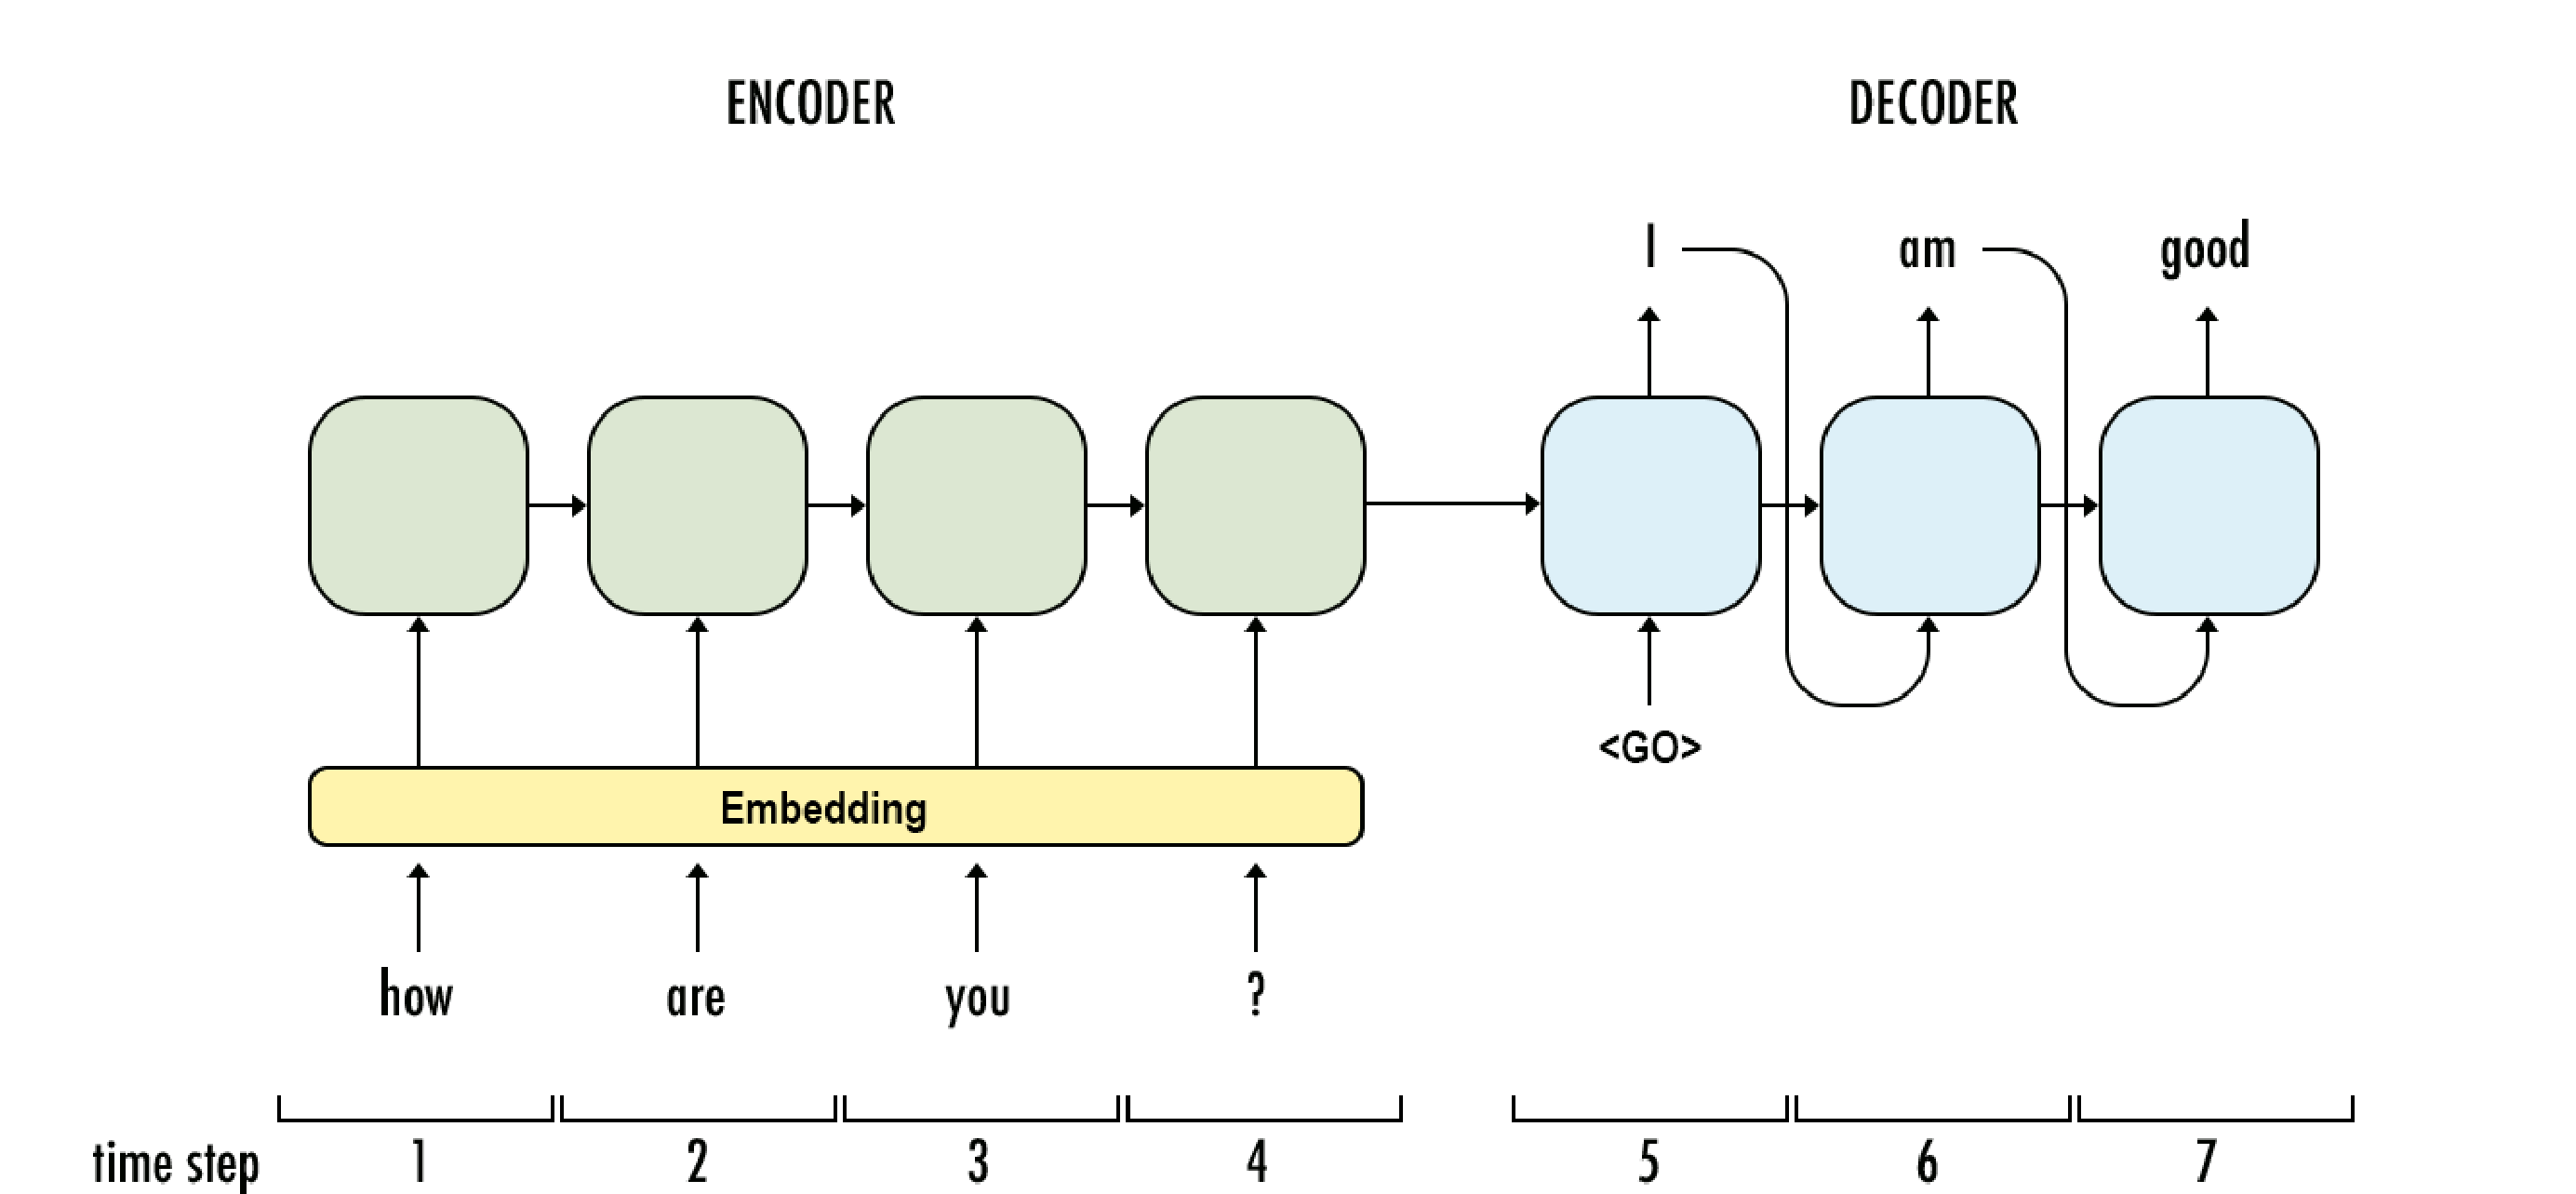
\includegraphics[width=\linewidth,keepaspectratio=true]{./figs/s2s-pdf}
		\else
		\includegraphics[width=\linewidth,keepaspectratio=true]{./figs/s2s-eps}
		\fi
		\caption{\small Schematic of a Seq2Seq \cite{s2s}}
		\label{bck:s2s}
	\end{minipage}
\end{figure}

Sequence-to-sequence (seq2seq) models introduced by Sutskever et al. , Cho et al. are a class of generative models that let us generate an output sequence when we are given an input sequence. They have found immense success in the fields of machine translation, speech recognition, question answering etc. 

Details about the latent space, and the probabilistic generative model.